% vim: set textwidth=78 autoindent:

\subsection{Plugin Creatore di Griglia}

% when the revision of a section has been finalized, 
% comment out the following line:
% \updatedisclaimer

Il creatore di griglia permette di creare una griglia di punti o poligoni per coprire un'area di interesse.
Tutte le unità di misura devono essere inserite in gradi decimali.
L'output è un file shape che può essere riproiettato al volo su altri dati.

\begin{figure}[ht]
\begin{center}
  \caption{Creare uno strato griglia \nixcaption}\label{fig:graticule}\smallskip
  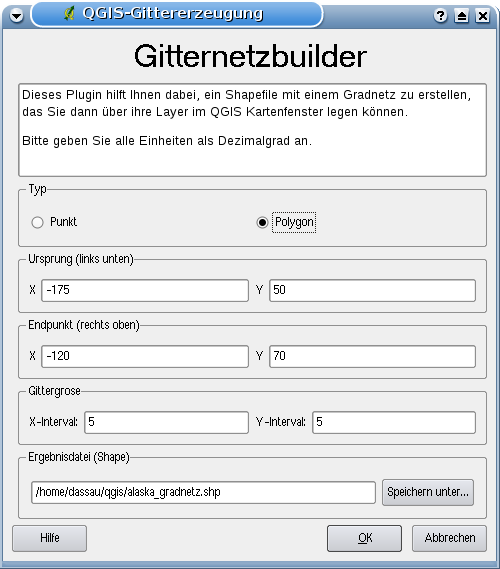
\includegraphics[clip=true, width=10cm]{grid_maker_dialog}
\end{center}
\end{figure}

Ecco un esempio di come c reare una griglia:

\begin{enumerate}
\item Lanciare QGIS, caricare il Plugin Creatore di Grtiglia nel Gestore dei Plugin (vedere Sezione 
\ref{sec:load_core_plugin}) e cliccare sull'icona \toolbtntwo{grid_maker}{Creatore di Griglia} che appare nella barra degli strumenti QGIS.
\item Scegliere il tipo di griglia che si vuole creare: punti o poligoni.
\item Inserire valori di latitudine e longitudine per gli angoli in basso a sinistra ed in alto a destra della griglia.
\item Inserire l'intervallo da usare nella costruzione della griglia. Si possono inserire valori diversi per le direzioni X e Y (longitudine, latitudine).
\item Scegliere il nome e la cartella in cui creare il file shape.
\item Cliccare \button{OK} per creare la griglia ed aggiungerla alla mappa.
\end{enumerate} 


